\subsubsection{Módulo de toma de decisiones $M_{12}$}

Como ya se ha visto el control de un sistema dependerá de las características y requisitos de cada aplicación, sin embargo, para este proyecto, se ha propuesto trabajar con dos tipos de control principalmente para regular las variables físicas y módulos que intervienen en el funcionamiento del compostador.

En un primer momento, se plantea utilizar control por PID para regular la temperatura, ya que para esta variable física se requiere de un control preciso y continuo, puesto que en esta ocasión, resulta indispensable mantener los valores de dicha variable en un rango ya establecido para este tipo de procesos, en este caso la temperatura, toma un rol muy importante en el compostaje , debido a que una temperatura adecuada permite una correcta proliferación de microorganismos.

Como el sistema contará con entrada de aire desde el exterior, la temperatura puede verse afectada por variaciones del entorno. Este es otro punto por el que control PID (Figura \ref{fg:PID}) resulta atractivo en esta situación, pues es capaz de adaptarse a estos cambios y perturbaciones, ya que ajusta continuamente los parámetros de control en función de la dinámica del sistema. 

\begin{figure}[h!]
            \centering
            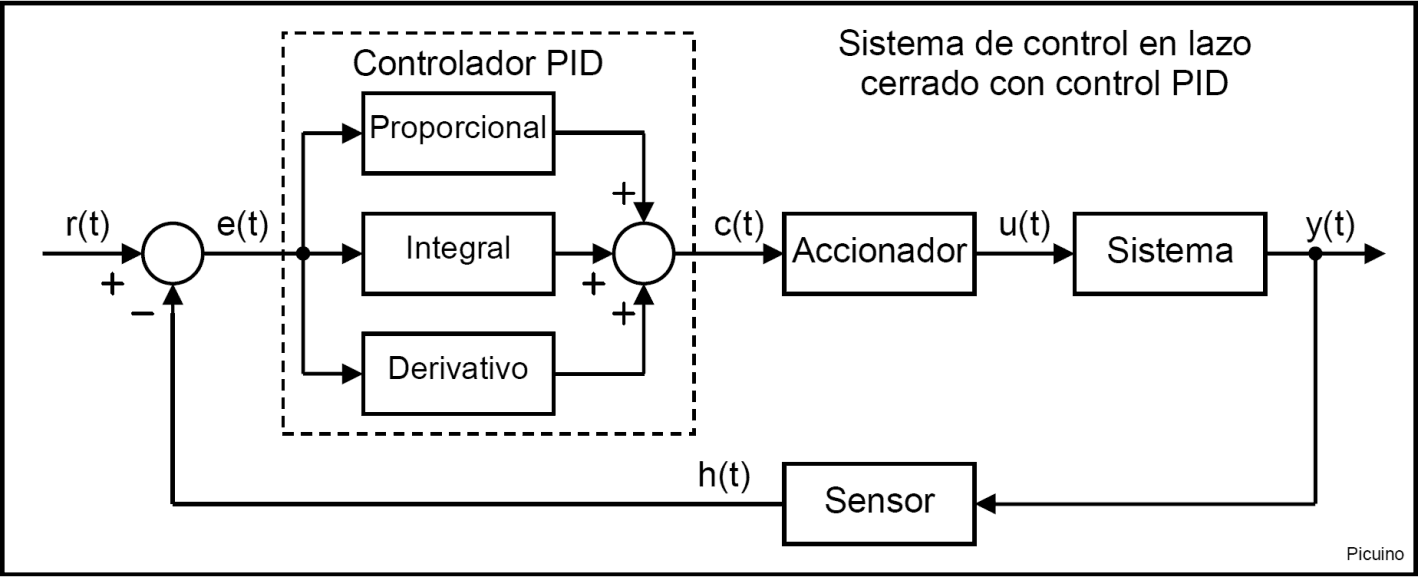
\includegraphics[scale=0.3]{images/Capitulo 4/3.1.1/PID_generico.png}
            \caption{Control PID}
            \label{fg:PID}
        \end{figure}

Como retroalimentación al PID se utilizará un sensor, encargado de realizar las mediciones de acuerdo con la variable física que se trate.
       
Por otro lado, en el caso del control del motor que moverá al eje del compostador y el control de humedad se propone utilizar el tipo ON/OFF (Figura \ref{fg:OnOff}) ya que no se requiere precisión en el movimiento del motor, tampoco es relevante conocer la posición en la que se queda el mismo. Sólo será requerido que el motor se active cuando sea necesario, de una forma rápida.

En el caso del control de humedad, también se ha optado por este tipo de control ya que se requerirá solamente encender y apagar una válvula, por lo que no demanda el uso de una técnica de control más sofisticada

\begin{figure}[h!]
            \centering
            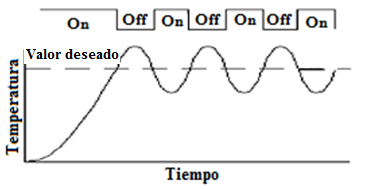
\includegraphics[scale=0.5]{images/Capitulo 3/3.1.2/OnOff.png}
            \caption{Control On/Off}
            \label{fg:OnOff}
        \end{figure}

\newpage